\documentclass[a4paper]{article}
%\usepackage{fullpage}
\usepackage{fancyhdr}
\usepackage[english,francais]{babel}
\usepackage[T1]{fontenc}
\usepackage[utf8]{inputenc}
\usepackage[pdftex]{graphicx}
\usepackage[a4paper]{geometry}
\usepackage{subfig}

%\renewcommand{\baselinestretch}{2}
\author{Brieuc \textsc{Daniel}, Océane \textsc{Lasserre}, Danchi \textsc{Li}, \\ Florent \textsc{Guiotte}, Frédéric \textsc{Becker}}
\title{Moteur de recherche d'images \\ \Large{Compte rendu de résultats}}
\pagestyle{fancy}

\begin{document}
\maketitle
\tableofcontents

\section{Introduction}

Le but de ce projet est de développer un moteur de recherche dans une base d'images. 

Le projet se divise en deux parties, une <<Offline>> et une <<Online>>. La première extrait et indexe des descripteurs sur une base de données
d'images. La deuxième extrait ce même type de descripteur sur une image requête, et cherche des
correspondances avec la base des descripteurs générée en <<Offline>>. La correspondance se fait à l'aide d'un 
algorithme de vote. Les meilleurs résultats sont alors affichés selon leur pertinence. 

Pour ce projet nous utiliserons deux types de descripteurs distincts.
Le descripteur {\em Speeded Up Robust
Features (SURF)} et le descripteur {\em Scale-invariant feature transform (SIFT)}.

\section{Tests et résultats}
\subsection{Tests avec différents descripteurs}

Sur une même base d'images, nous avons testé l'algorithme avec deux descripteurs différents.

\subsubsection{SURF}

La fonction SURF donne les résultats de la figure \ref{surf}.

\begin{figure}[!ht]%htp]
  \centering
  \subfloat[SURF - knn]{\label{surf:knn}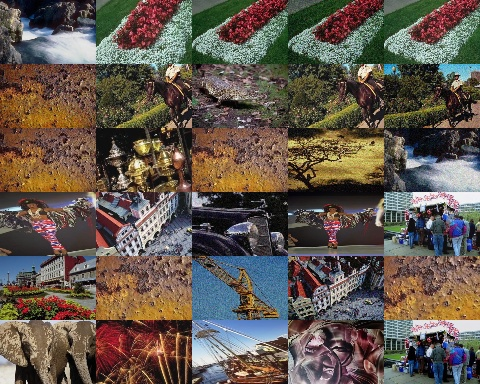
\includegraphics[width=0.49\textwidth]{img/KMeansIndex/knn/corel_0000000303_512_COREL_SURF.jpg}}
  \hspace{0.01\textwidth}
  \subfloat[SURF - Spheric]{\label{surf:spheric}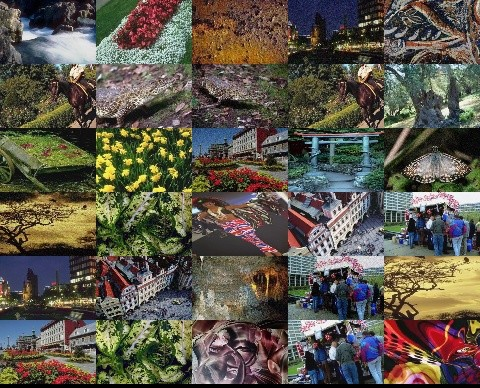
\includegraphics[width=0.49\textwidth]{img/KMeansIndex/radius/corel_0000000303_512_COREL_SURF.jpg}}
  \caption{Résultats avec SURF via une recherche knn (\ref{surf:knn}) et sphérique (\ref{surf:spheric}).}
  \label{surf}
\end{figure}

L'image en haut à gauche de chaque figure correspond à l'image requête retrouvée. Les images suivantes sont
classées de la plus pertinente à la plus eloignée (de gauche à droite).
On observe que les résultats sont éloignés de l'image requête. 

L'image requête est bien retrouvée mais les autres images obtenues ne sont pas pertinentes et les images les
plus proches <<instinctivement>> ne sont pas retrouvées. 
Le type de recherche (knn ou sphérique) a une influence importante sur les résultats mais ne semble pas les rapprocher de l'image requête. 

\subsubsection{SIFT}

La fonction SIFT donne les résultats de la figure \ref{sift} (sur les mêmes images requêtes que précédemment).

\begin{figure}[!ht]%htp]
  \centering
  \subfloat[SIFT - knn]{\label{sift:knn}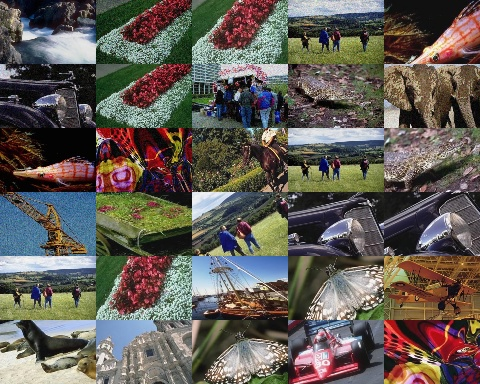
\includegraphics[width=0.49\textwidth]{img/KMeansIndex/knn/corel_0000000303_512_COREL_SIFT.jpg}}
  \hspace{0.01\textwidth}
  \subfloat[SIFT - Spheric]{\label{sift:spheric}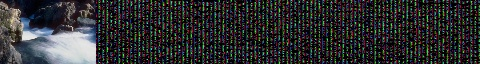
\includegraphics[width=0.49\textwidth]{img/KMeansIndex/radius/corel_0000000303_512_COREL_SIFT.jpg}}
  \caption{Résultats avec SIFT via une recherche en knn (\ref{sift:knn}) et sphérique (\ref{sift:spheric}).}
  \label{sift}
\end{figure}

L'image en haut à gauche de chaque figure correspond à l'image requête retrouvée. Les images suivantes sont
classées de la plus pertinente à la plus eloignée (de gauche à droite).

La pertinence des résultats ici est la même que pour les descripteurs SURF. En revanche pour une recherche sphérique, 
si les images sont trop éloignées pour être conservées alors seule l'image requête est trouvée (comme dans
notre cas, figure \ref{sift:spheric}).
Le nombre de <<vrais positifs>> n'est pas amélioré mais cela diminue 
le nombre de <<faux positifs>>. Selon le type de recherche, cela peut être, ou non, un avantage.

\subsection{Tests sur différentes méthodes d'indexation}

Nous avons comparé trois méthodes d'indexation différentes~:

\begin{itemize}
    \item {\em Linéaire}, on effectue une recherche linéaire de l'index, en mode {\em brute-force}.
    \item {\em KDTree}, on effectue la recherche en parallèle dans l'index organisé en plusieurs ensembles aléatoires de kd-trees.
    \item {\em KMeans}, l'index construit est organisé en arbre k-means hiérarchique
\end{itemize}

Nous avons évalués ces méthodes en nous aidant de deux facteurs, la rapidité et la précision.
Sur ces points, l'index linéaire est plus rapide que le KDTree qui lui même est plus rapide que le KMeans.
Tandis que pour la précision, le meilleur est le KMeans, suivi par le KDTree, puis l'index linéaire.
Pour conclure, les index sont proportionnellement précis par rapport à leur lenteur.


% speed: linearIndex > KDTreeIndex > KmeansIndex
% accuracy: linearIndex < KDTreeIndex < KmeansIndex
% sift flann match distance is very big

\subsection{Tests sur différentes bases d'images}

Avec le même descripteur, nous avons testé l'algorithme sur la base d'images {\em NISTER}. Cette base
d'images propose des échantillons de transformation\footnote{Rotations, translations, bruitage\ldots} sur quelques images.
Les résultats sont visibles figure \ref{db}. Les résultats semblent plus pertinents sur cette base d'images,
surtout avec les descripteurs SIFT (cf. figure \ref{db:sift}).

\begin{figure}[!ht]%htp]
  \centering
  \subfloat[SIFT]{\label{db:sift}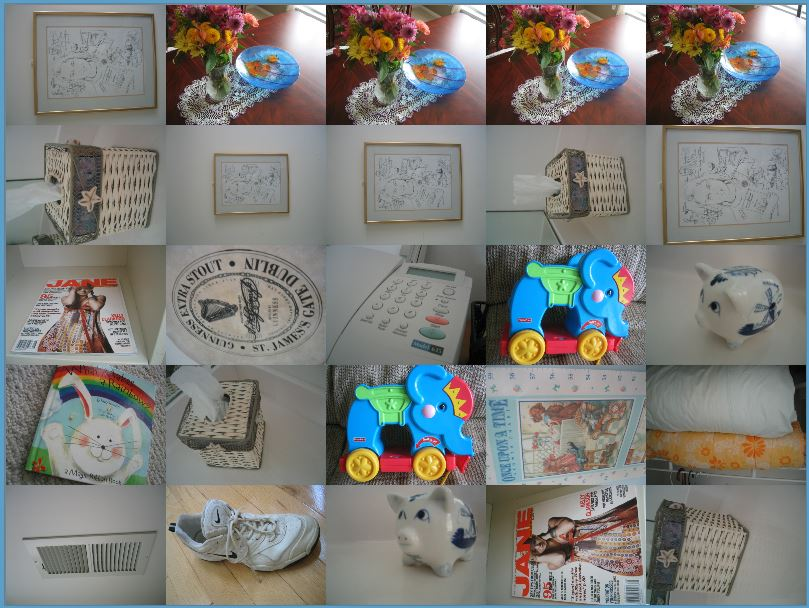
\includegraphics[width=0.49\textwidth]{img/sift_knn=25_linear.JPG}}
  \hspace{0.01\textwidth}
  \subfloat[SURF]{\label{db:surf}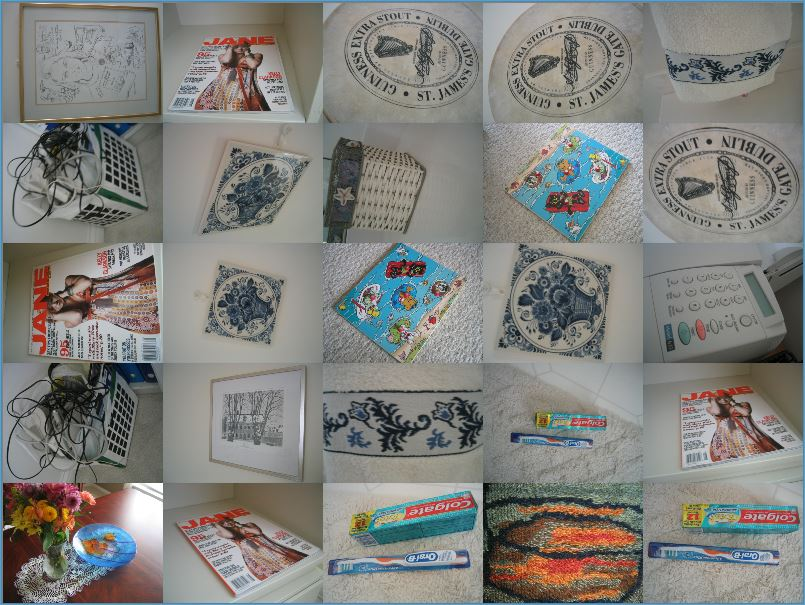
\includegraphics[width=0.49\textwidth]{img/SURF_knn=25_linear.JPG}}
  \caption{Résultats de l'algorithme avec la base d'images NISTER}
  \label{db}
\end{figure}

\section{Conclusion}

Notre algorithme permet dans tous les cas testés de retrouver l'image requête. Néanmoins, une très légere variation dans l'image peut influencer 
sa position dans les résultats de façon très importante. 
De plus, selon le cas et le type de résulats souhaités (précis ou larges), on peut adapter le choix du descripteur.
Pour améliorer nos résultats, il faudrait ajouter des traitements en plus sur les images, par exemple de type comparaison d'histogrammes, pour affiner la recherche.
\end{document}

